\section{Parallelization}
\label{sec:parallelization}

The ease with which an algorithm can be parallelized and its performance is important for handling large-scale graphs in emerging applications, where graphs with millions (or more) vertices have become quite common. In this section we describe how our exact algorithm can be parallelized, and show its performance on shared-memory architectures. The heuristic can be parallelized following a similar procedure.

%We here describe the parallelization procedure for both shared and distributed memory architecture. 
As explained in Section \ref{sec:algorithms}, the $i$th iteration of the {\em for} loop, in both the exact and the heuristic algorithm, computes the size of the largest clique that contains the vertex $v_i$. Since our algorithm doesn't enforce any strict order in which the vertices have to be processed, these iterations are essentially computationally independent. In other words, the sizes of the largest cliques containing different vertices can be computed concurrently by different computational units. However, different computational units might discover maximum cliques of different sizes, and for the pruning steps to be most effective, it is important that all units are updated about the globally largest maximum clique size among all units. While this is not a problem in a shared-memory programming model, since the maximum clique size can be stored in a shared memory location which is accessible to all the processing units, it might not be as trivial to handle in distributed memory models. For the distributed case, the effects of pruning could, however, be tolerably compromised in order to enable the parallel computation. This can, for example, be done by using the most recent value of the maximum clique size for pruning, and updating this value by having synchronization steps at regular intervals.

We implemented a shared-memory algorithm based on the procedure described above using OpenMP. Since the global value of the maximum clique is shared by all processing units, we embed the updating of the maximum clique, i.e. Line \ref{critical} of Algorithm \ref{alg:mClq}, into a {\it critical} section, which is an OpenMP feature that enforces a lock, allowing only one thread to make the update at a time. We used  dynamic load scheduling, since different vertices might return different sizes of maximum clique, hence computation time, so would work best for our case.

We performed experiments on the same graphs listed in the testbed described in Section \ref{sec:experiments}. For these, we used a Linux workstation running 64-bit version Red Hat Enterprise Linux Server release 6.2, with six 2.00 GHz Intel Xeon E7540 processors. Each processor has six cores, each with 32 KB of L1 and 256 KB of L2 cache, and each processor shares a 18 MB L3 cache.  Implementation was in C++ using OpenMP and compiled with gcc (version 4.4.7) using the -O3 optimization flag.


\begin{figure}
  \centering
    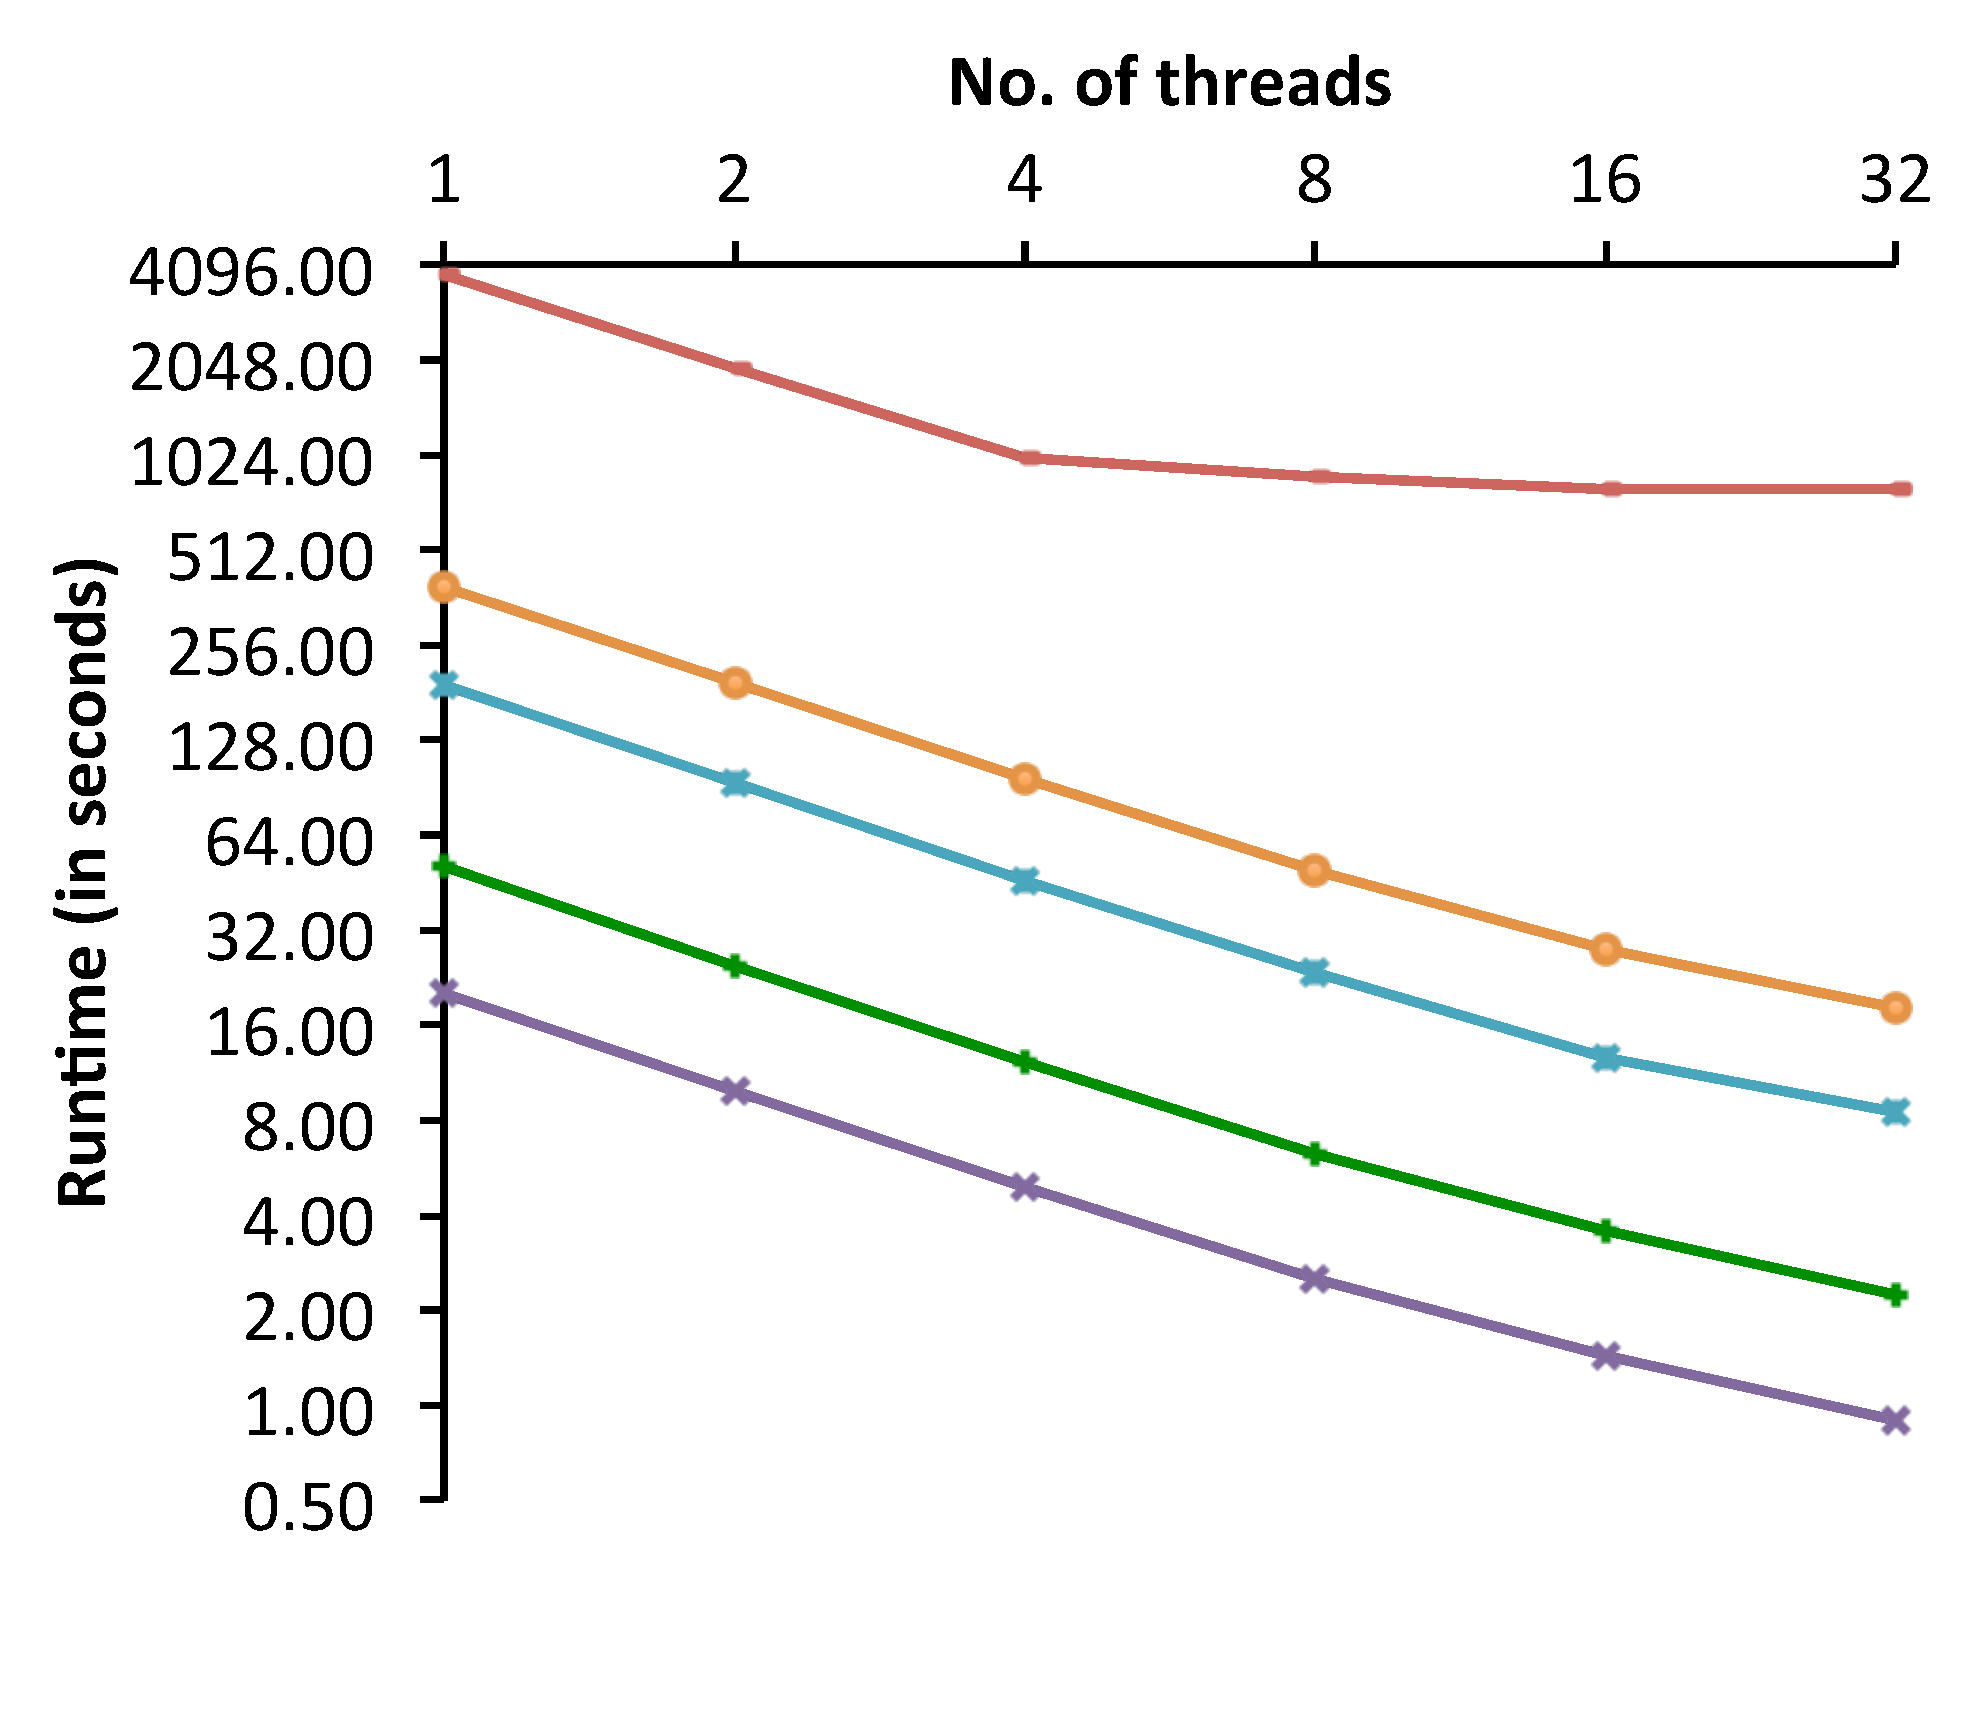
\includegraphics[scale=0.17]{parallel_realworld_timing.pdf}
    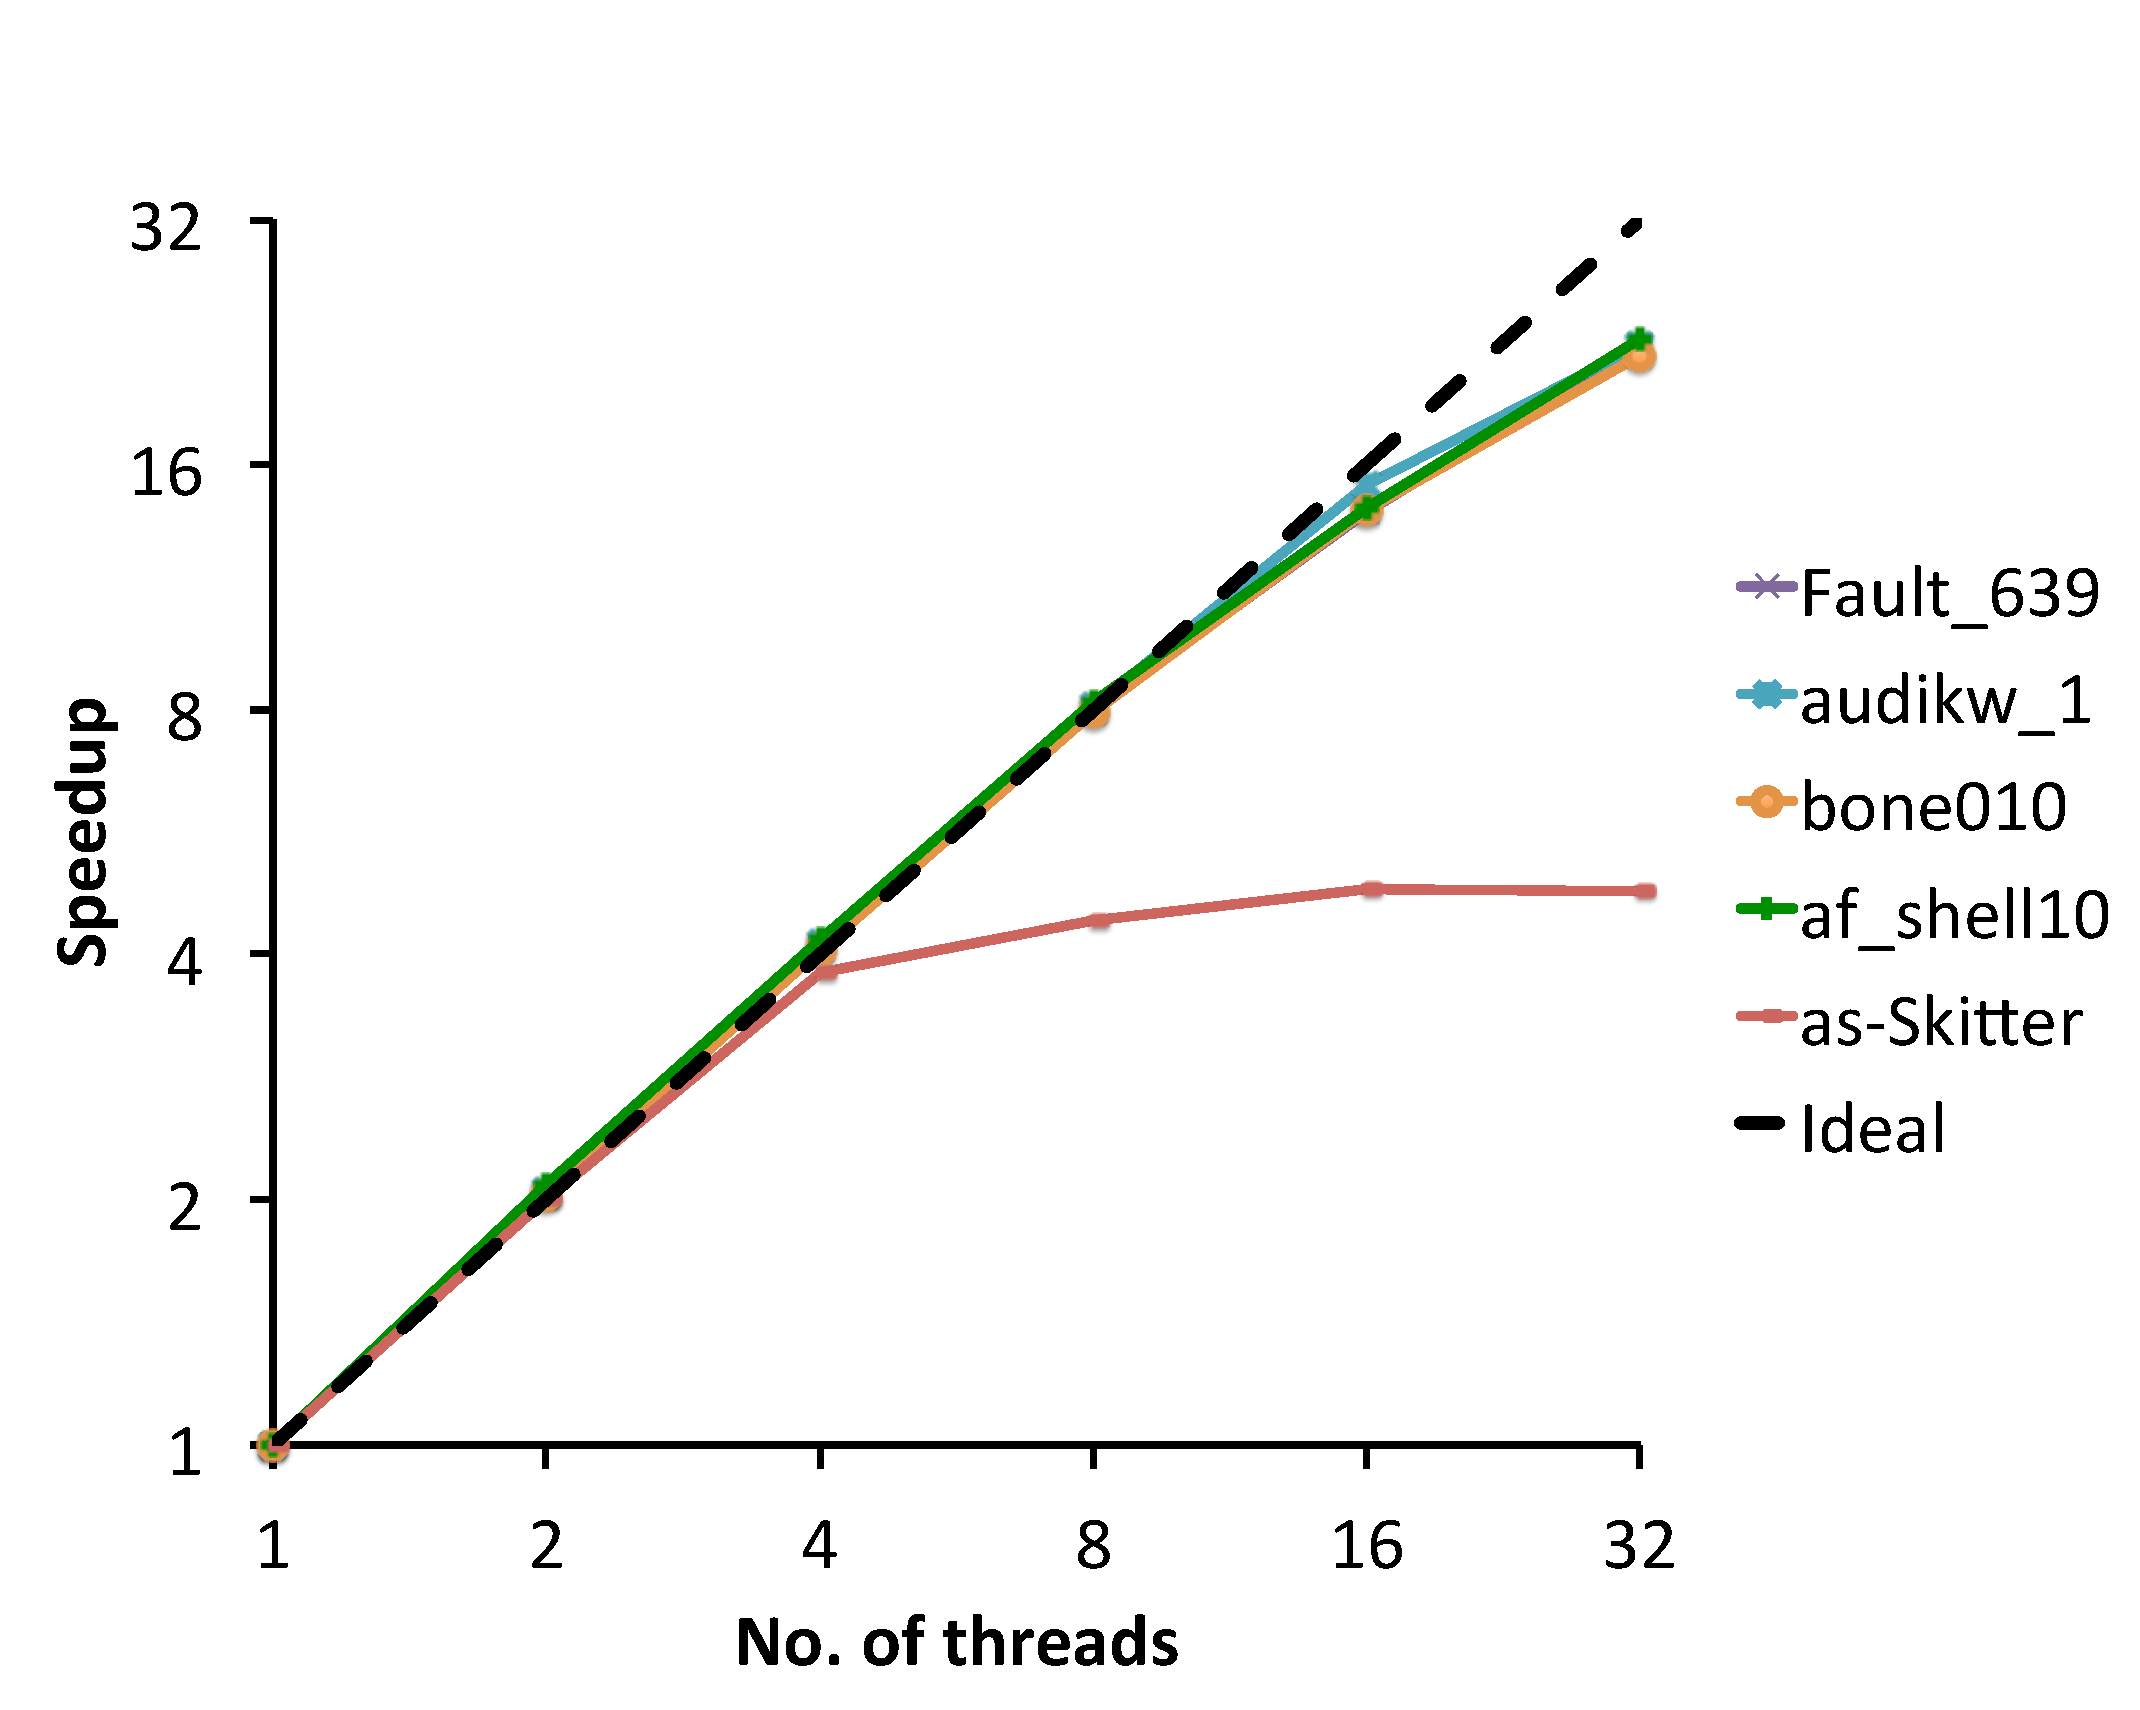
\includegraphics[scale=0.17]{parallel_realworld_speedup.pdf}
    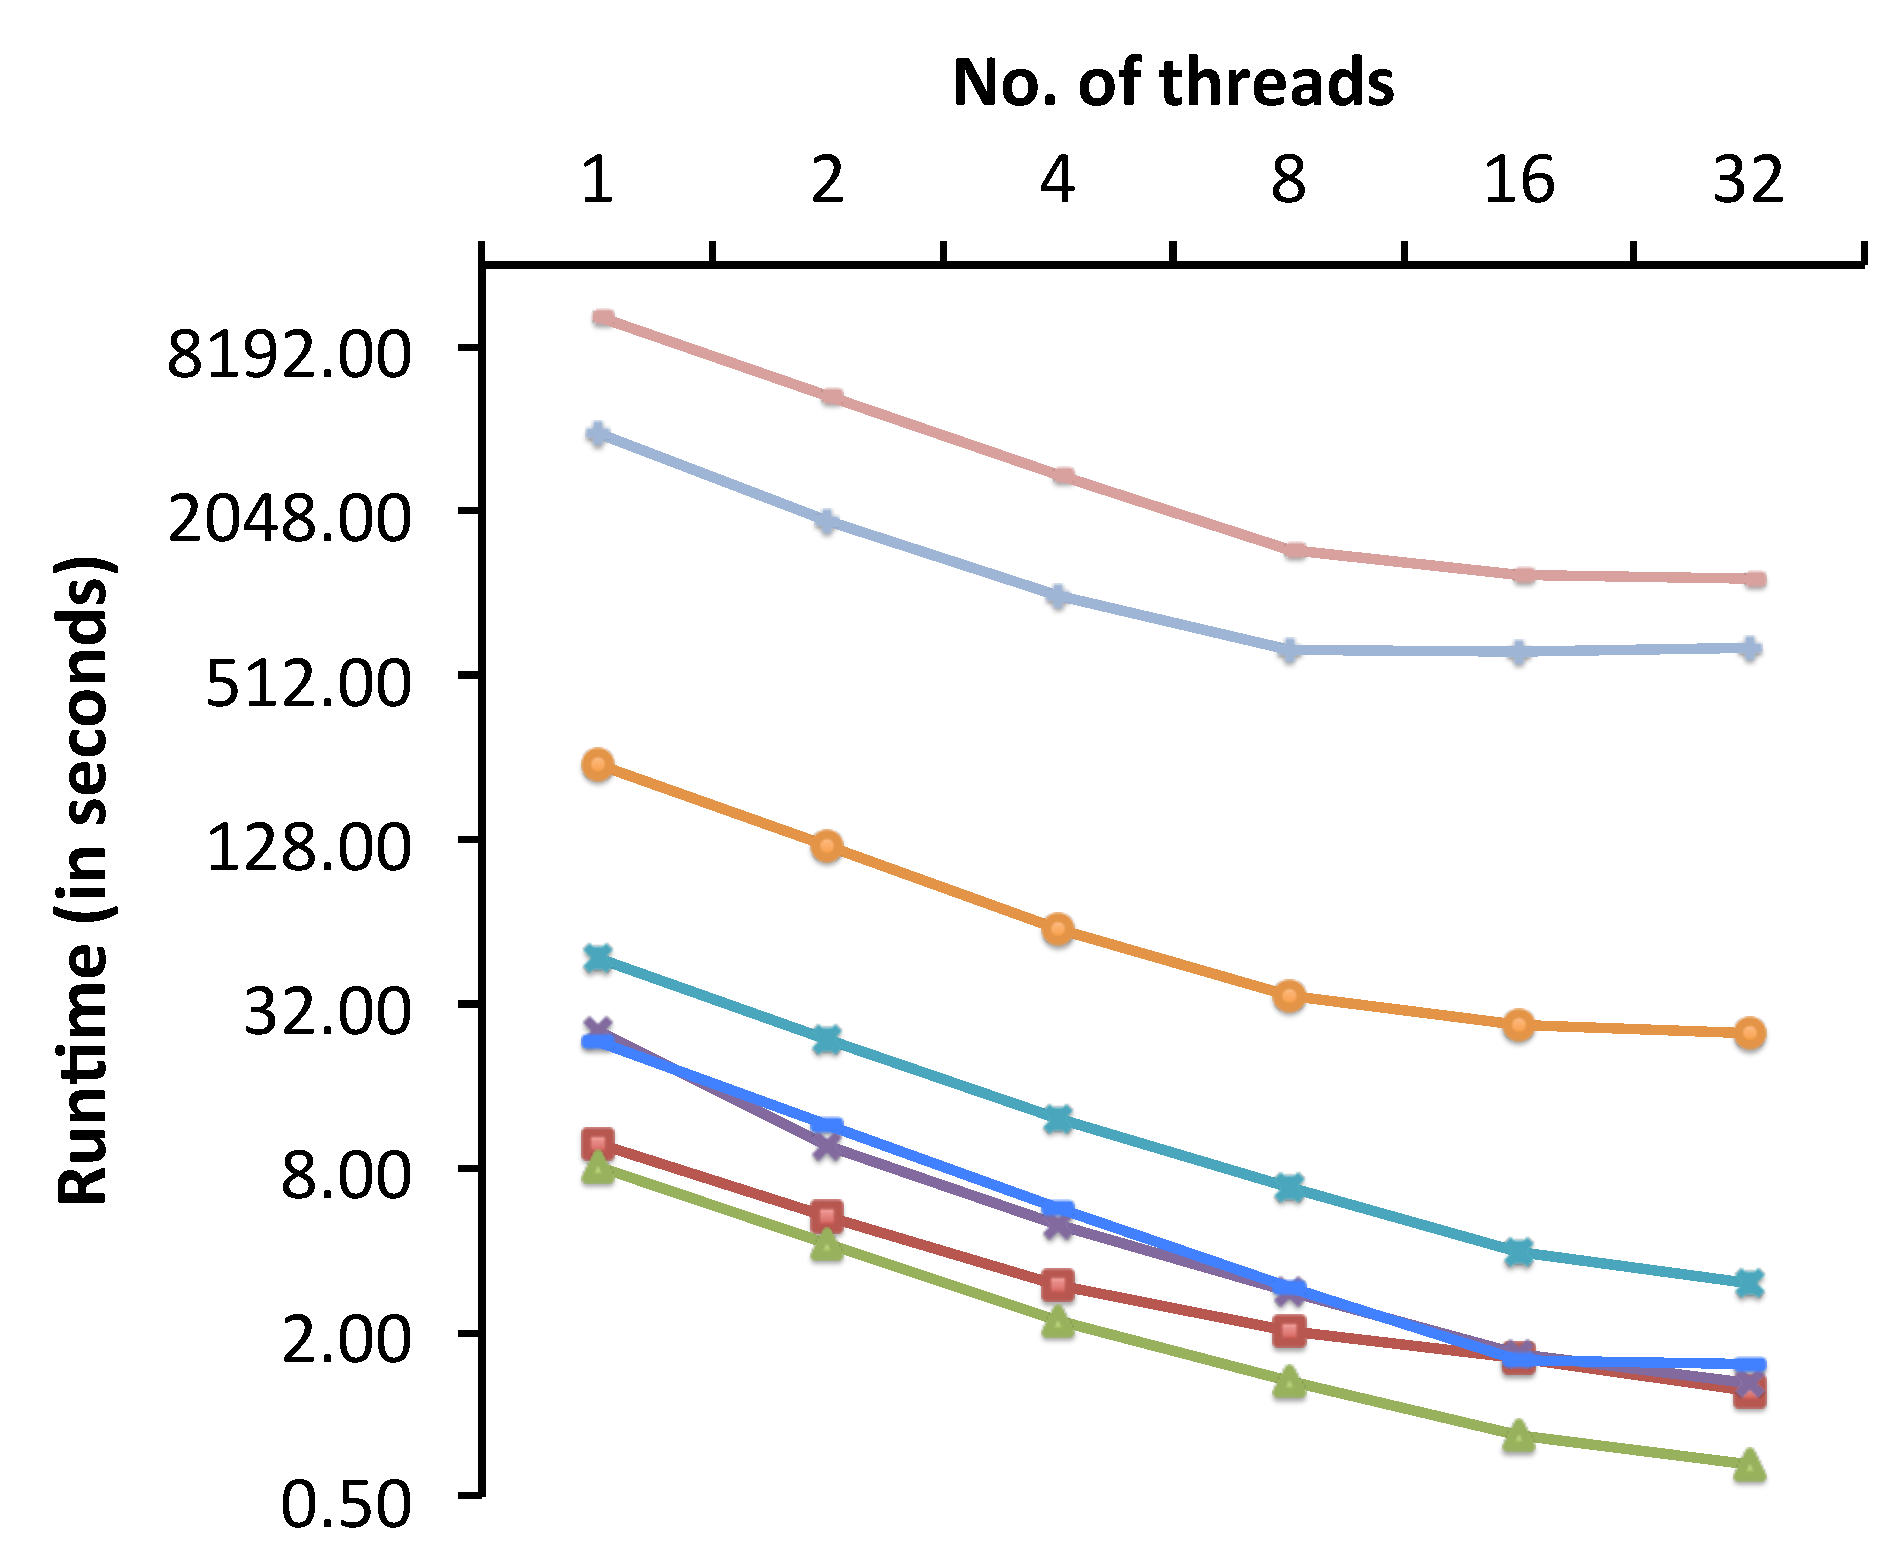
\includegraphics[scale=0.17]{parallel_other_timing.pdf}
    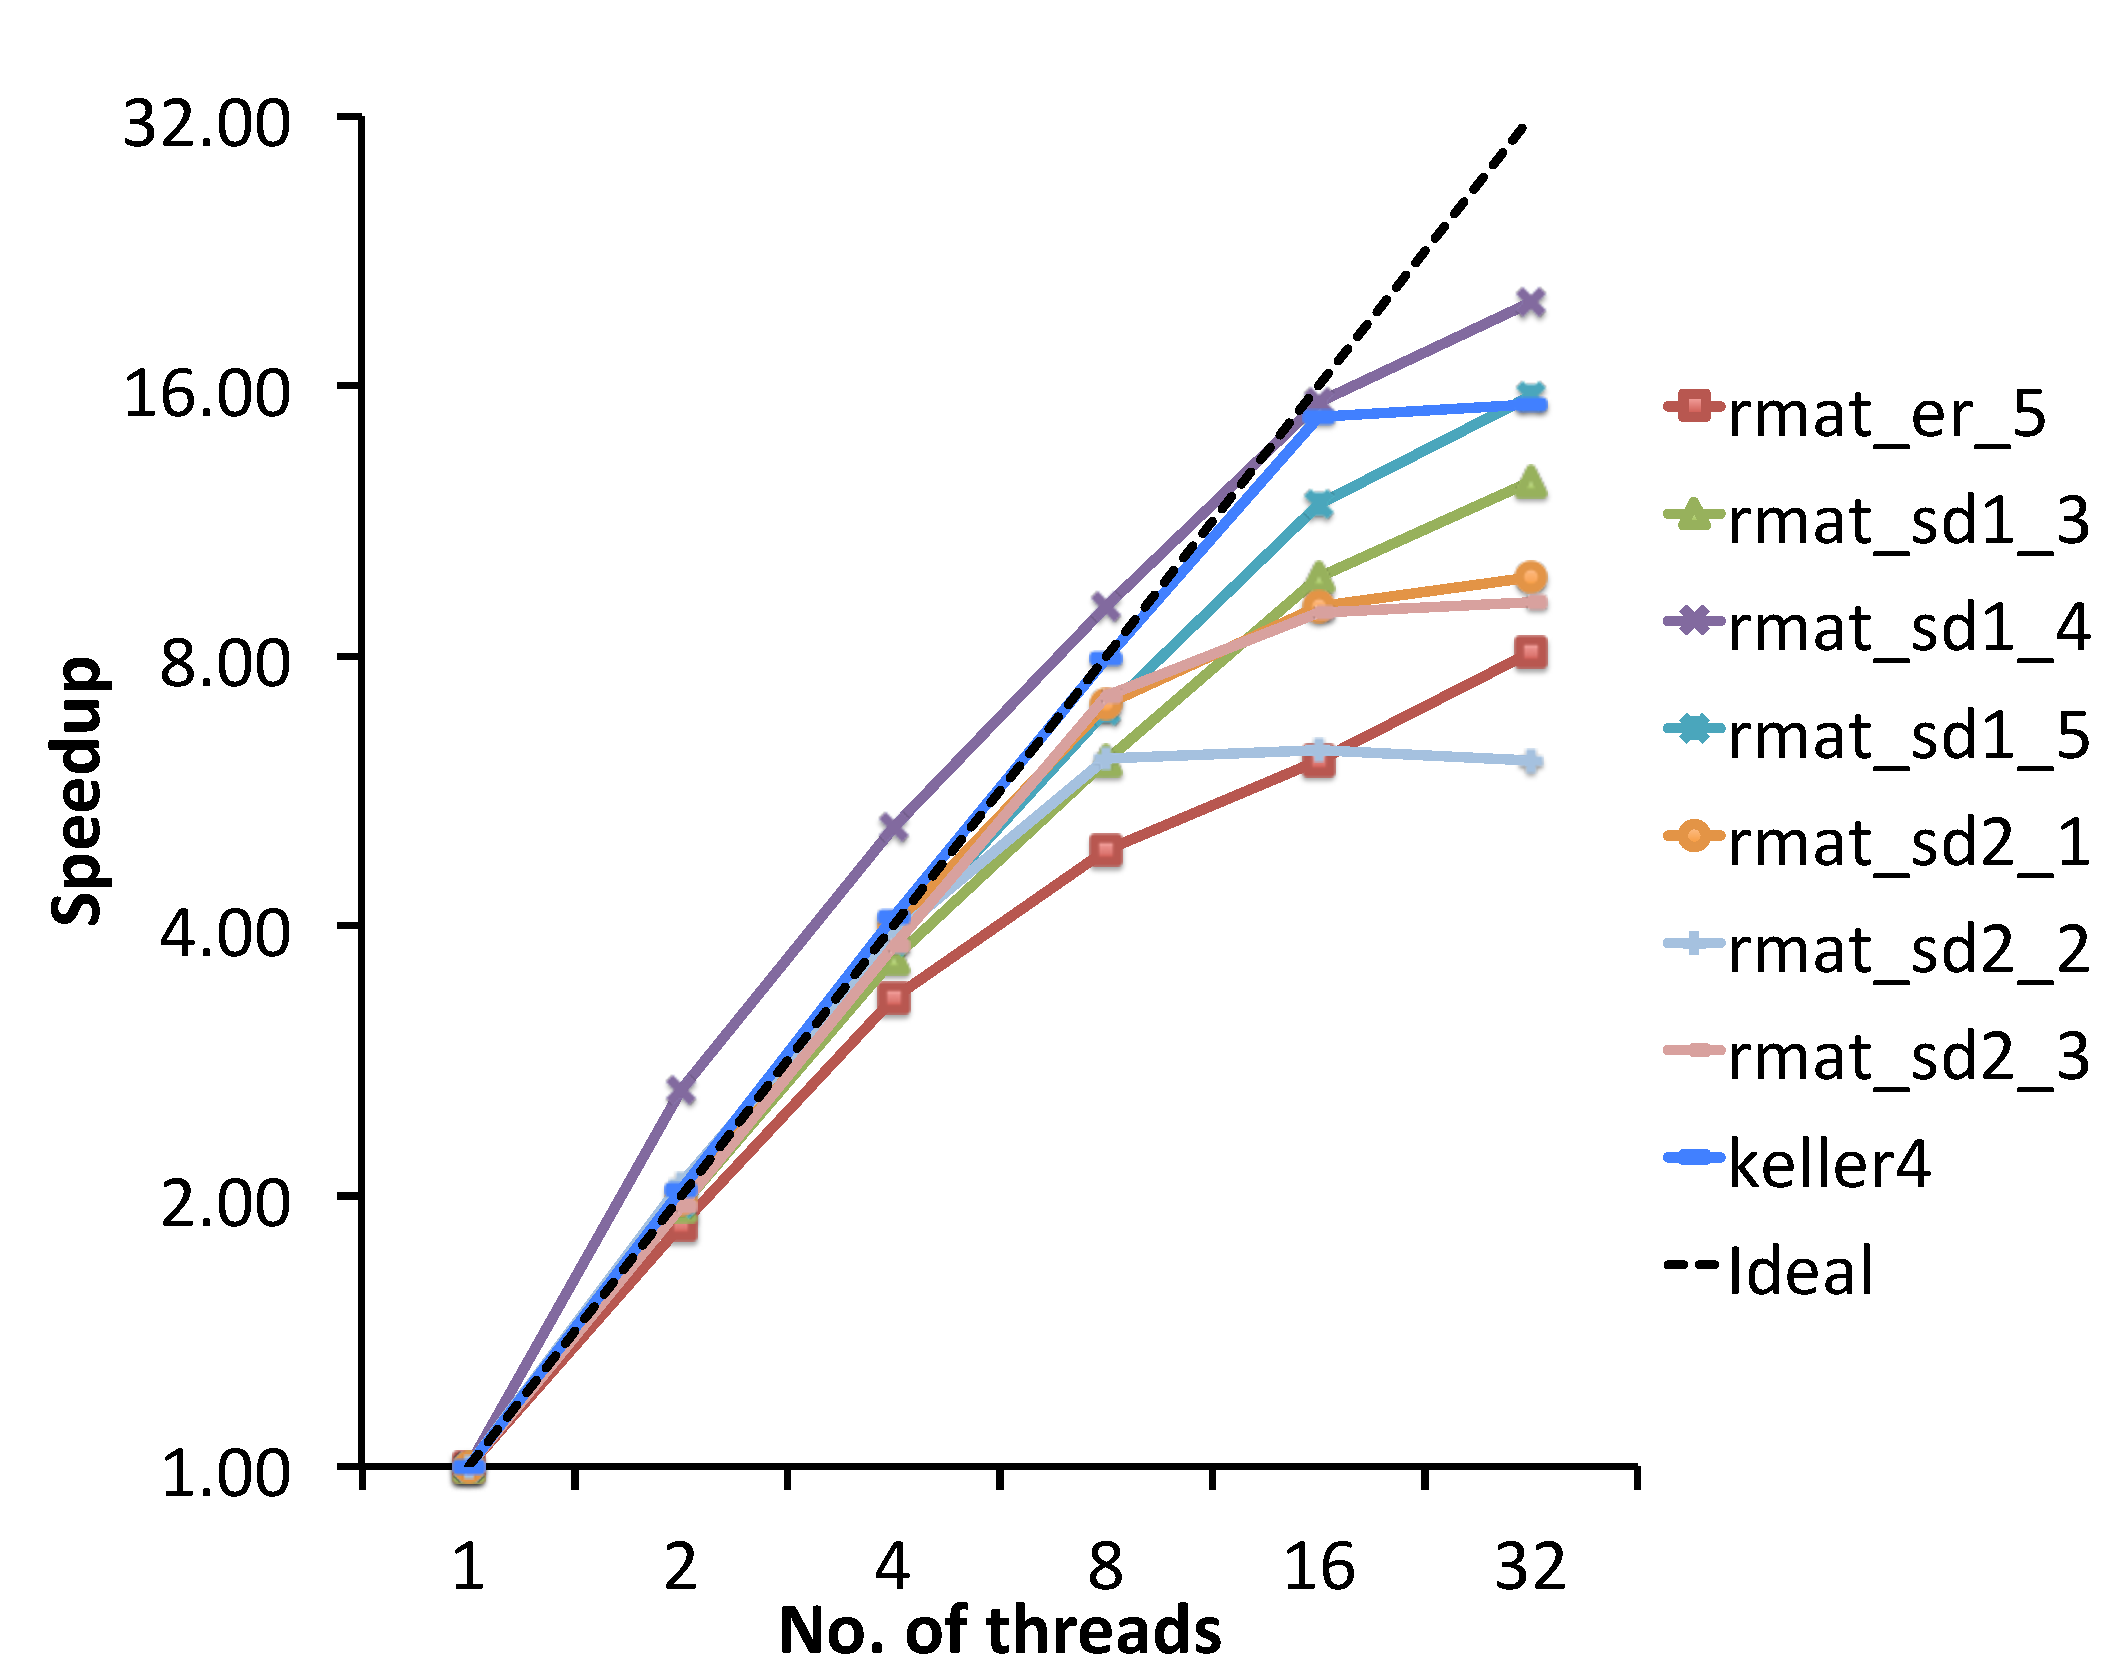
\includegraphics[scale=0.17]{parallel_other_speedup.pdf}
    
%%\vspace{-30pt}
 \caption{Performance (timing and speedup plots) of shared-memory parallelization on graphs in the test-bed. Graphs whose sequential runtime is less than 5 seconds are omitted. The top set of figures show performance on real-world graphs, whereas the bottom set show for the others.}
\label{fig-parallel_perf}
\end{figure}


Figure \ref{fig-parallel_perf} shows the timings and speedups we obtained for the real-world and other graphs separately. We omitted graphs whose sequential runtimes were less than 5 seconds as they were too low to measure, and are not be good test cases for measuring parallelization performance. For the real-world graphs, one can see from the figure that we obtained near-linear scaling of runtimes and speedups up to 16 threads for most graphs. The only exception is {\emph as-Skitter}. It's relatively poorer scaling is probably due to the fact that this instance has a relatively large maximum clique, and hence the core(s) which compute(s) it spends relatively large amount of time computing it, while the other cores which have processed the remaining nodes remain idle after completion. For the other instances, the maximum speedups we obtain for 32 cores/threads is around 22$\times$. 
For the other instances, we can see the scaling of the runtime and speedups vary based on the instance. We observe super-linear scaling for a couple of instances. For the others, it scales fairly well till 8 threads, and deteriorates with higher number of threads. The speedups we obtain are anywhere between 6$\times$ - 20$\times$.





%The effects of pruning could, although, be tolerably compromised in order to enable the parallel computation by allowing the processors to use the locally computed maximum clique value as the lower bound for pruning until regular synchronization steps, during which it is updated to the global value of the maximum clique across all processors.

%When done in parallel, the for loop in Algorithm \ref{alg:mClq} can be distributed among different $p$ computational units which can compute different values for $max$ in parallel. In the next step, a reduce operation can be used to find the maximum of the $p$ values.

%In this section we show the results of parallelization of our exact algorithm on shared memory architectures. In our algorithm, there is no dependency or strict order in which the vertices have to be computed unlike other previous algorithms. The sizes of the largest cliques containing different vertices can be computed mostly independently, and thus can be done in parallel by different computational units.


%\begin{figure}
%        \centering
%        \begin{subfigure}[b]{0.5\textwidth}
%                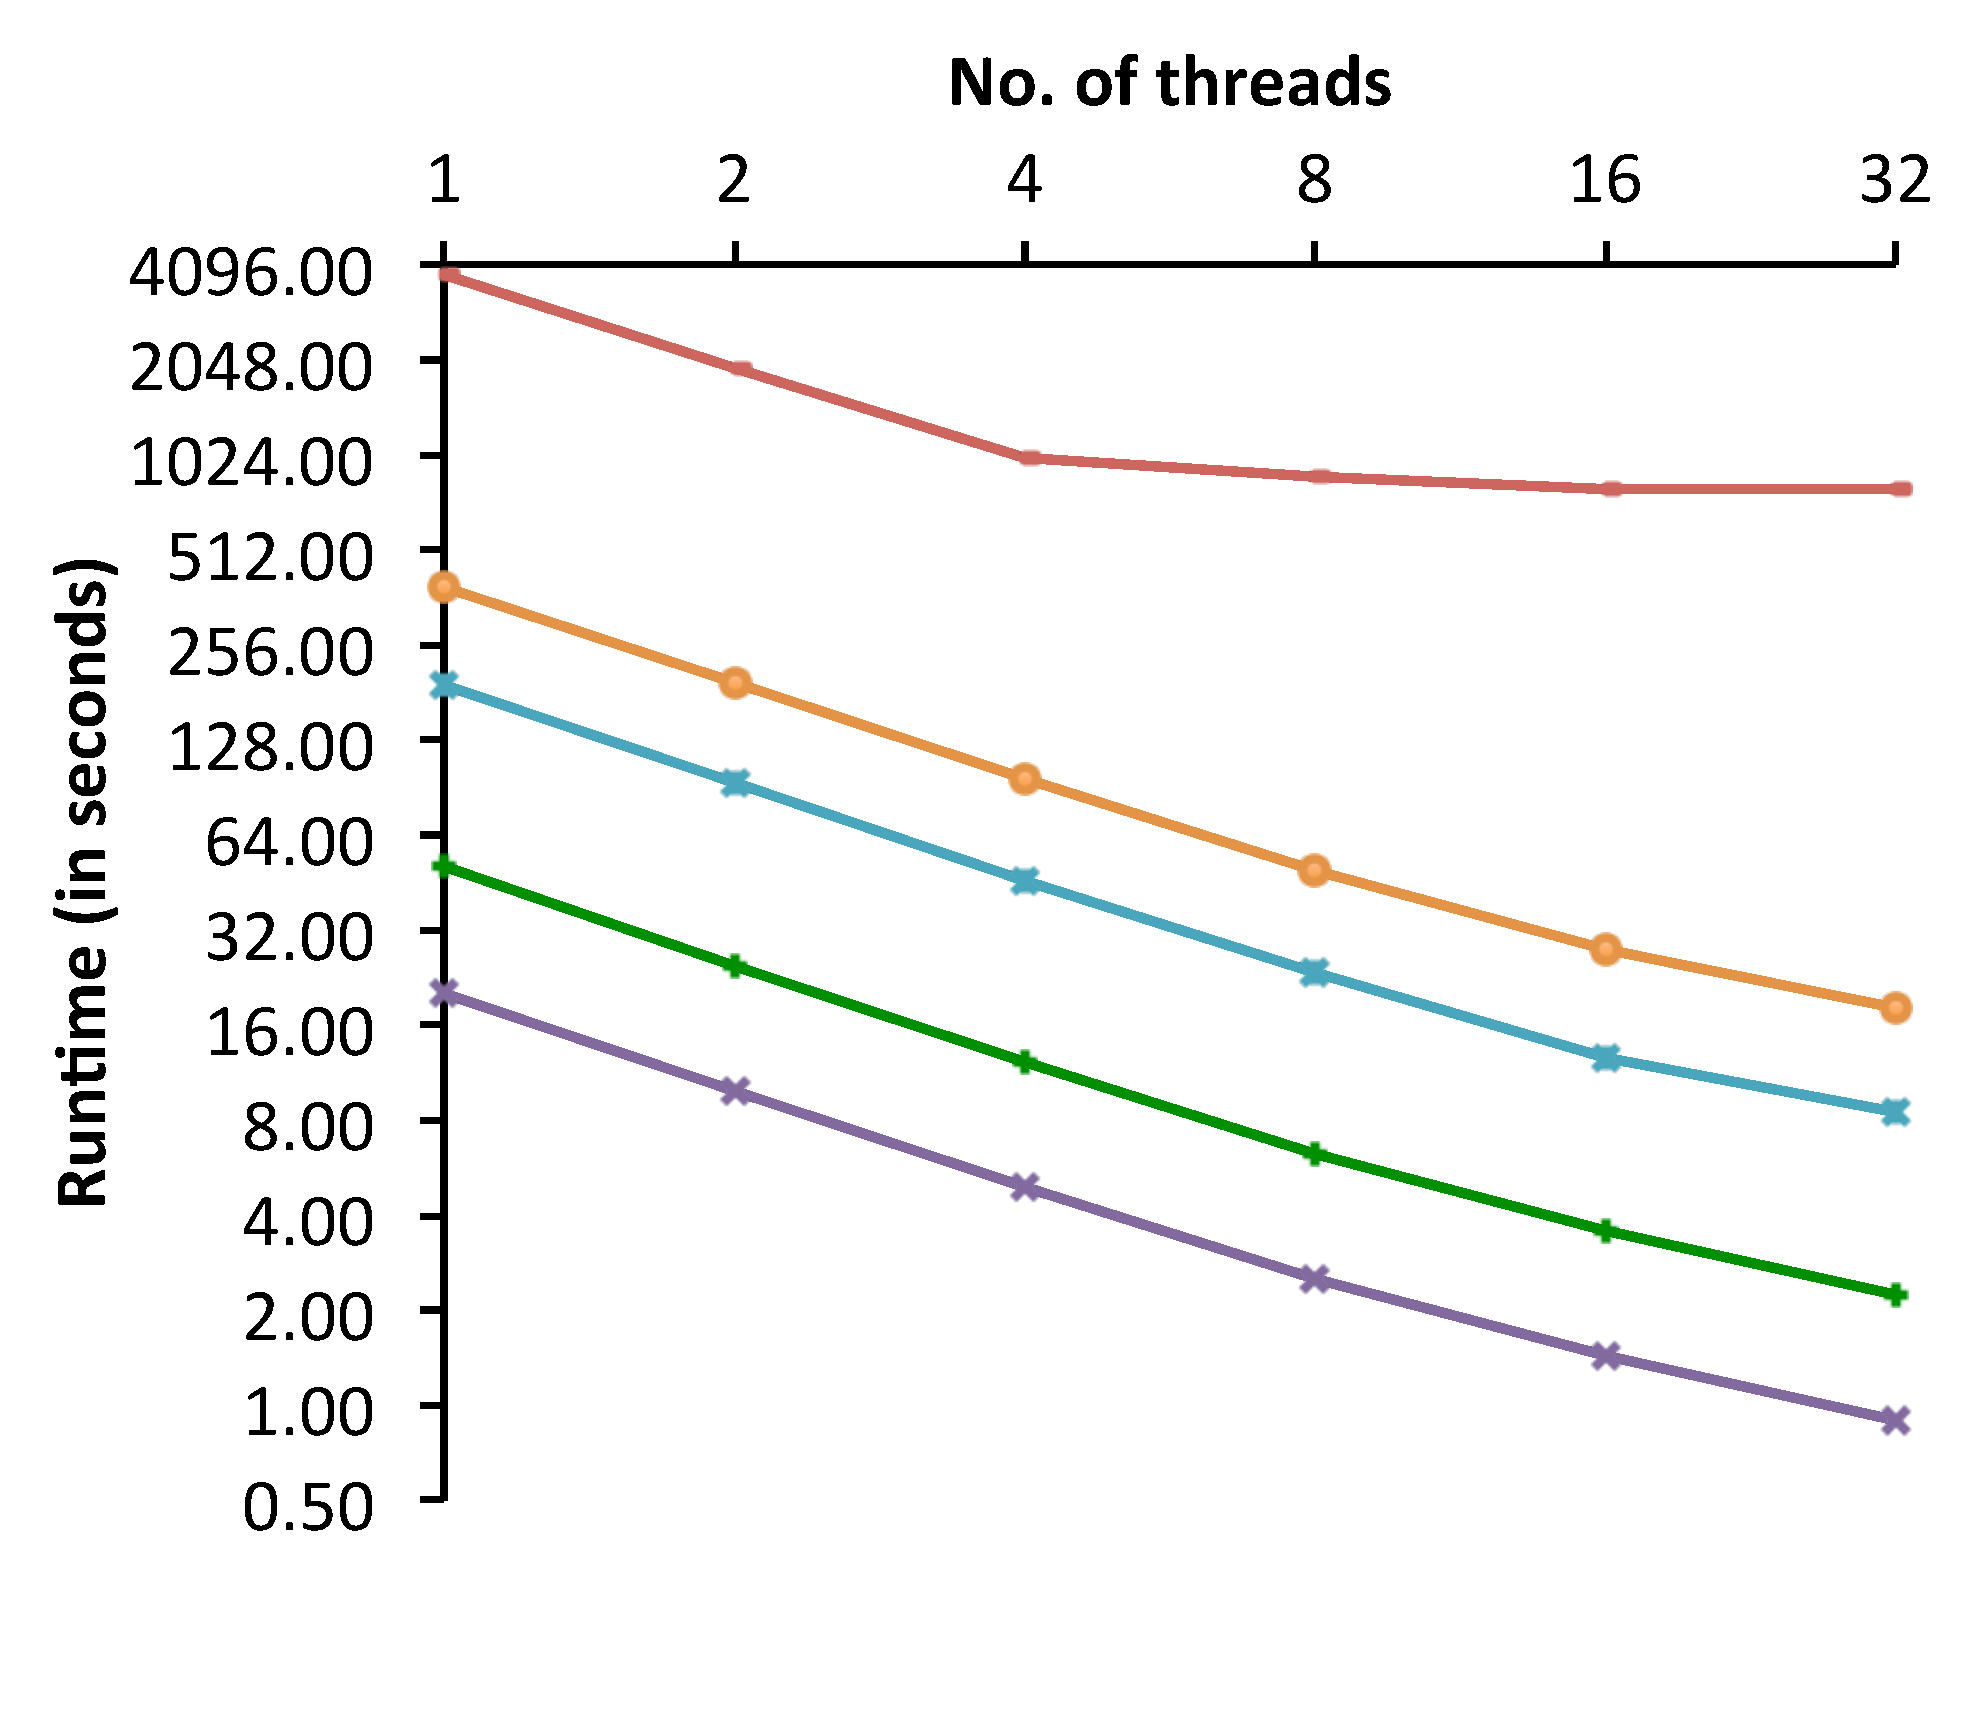
\includegraphics[width=\textwidth]{parallel_realworld_timing.pdf}
%                \caption{Timing results}
%                \label{fig:timing_realworld}
%        \end{subfigure}%
%        ~ %add desired spacing between images, e. g. ~, \quad, \qquad etc.
%          %(or a blank line to force the subfigure onto a new line)
%        \begin{subfigure}[b]{0.5\textwidth}
%                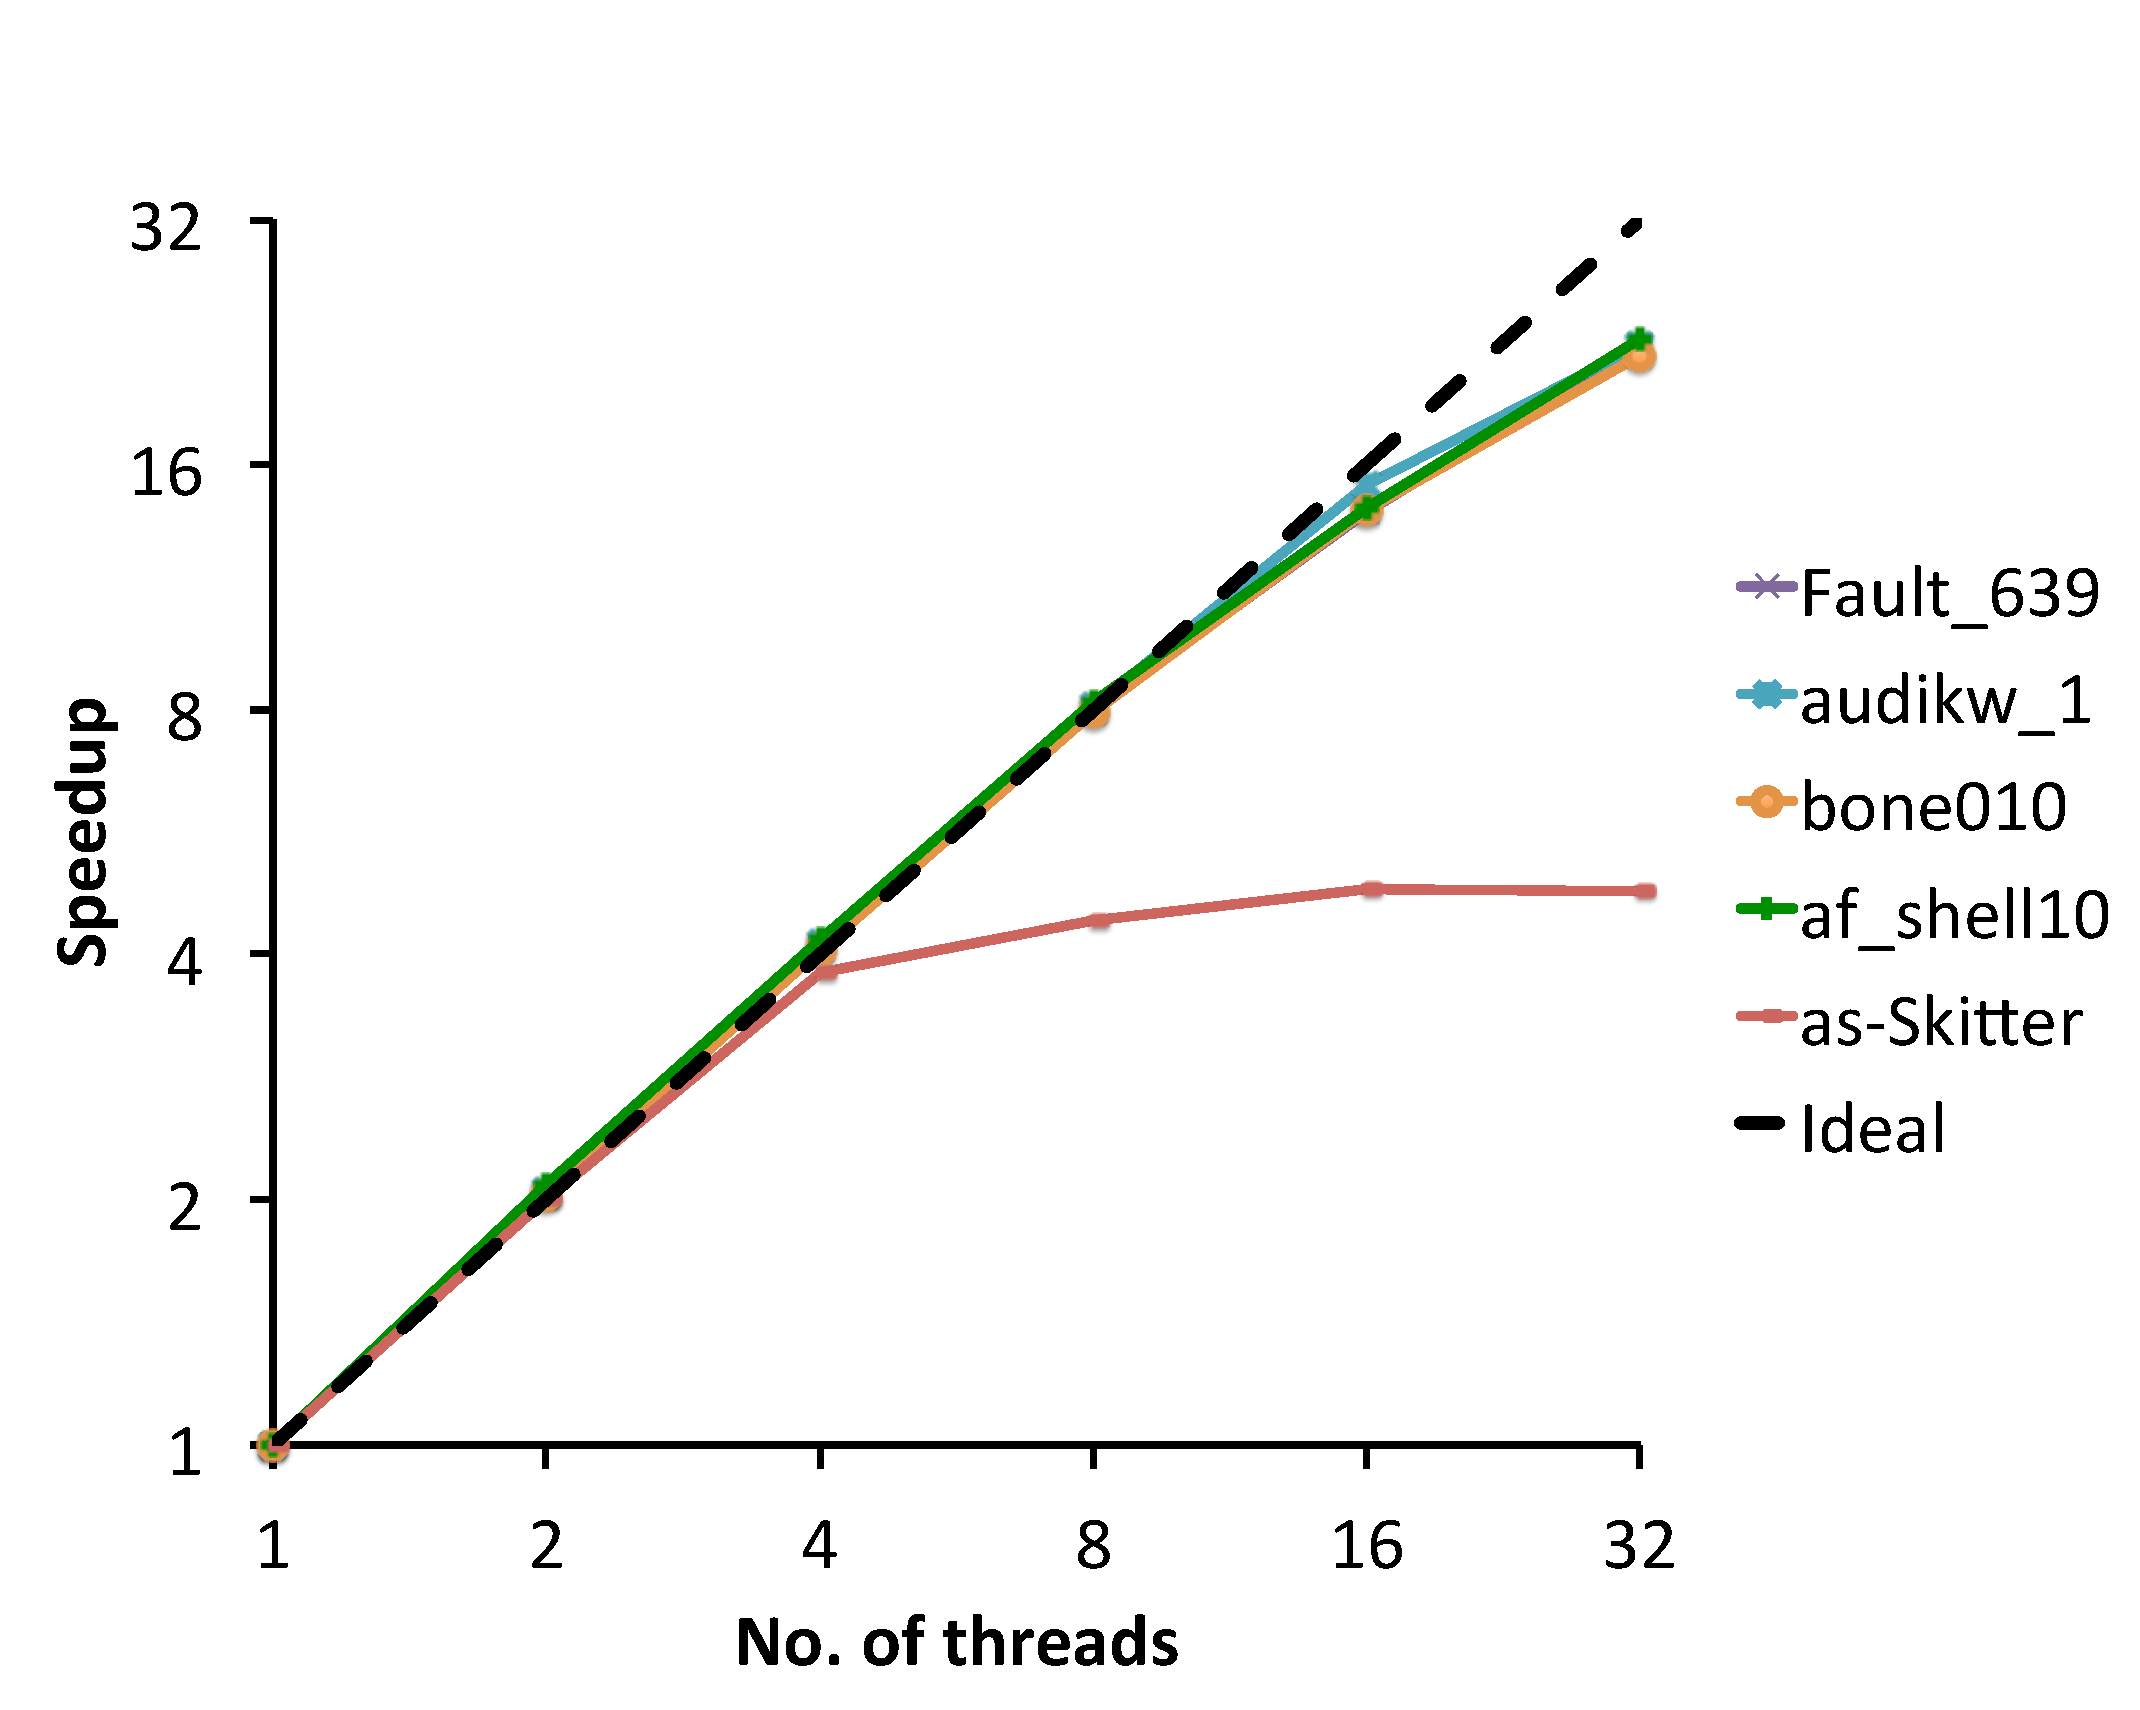
\includegraphics[width=\textwidth]{parallel_realworld_speedup.pdf}
%                \caption{Speedup results}
%                \label{fig:speedup_realworld}
%        \end{subfigure}
%        \caption{Performance of shared-memory parallelization on real-world graphs}\label{fig:animals}
%\end{figure}
%
%
%\begin{figure}
%        \centering
%        \begin{subfigure}[b]{0.5\textwidth}
%                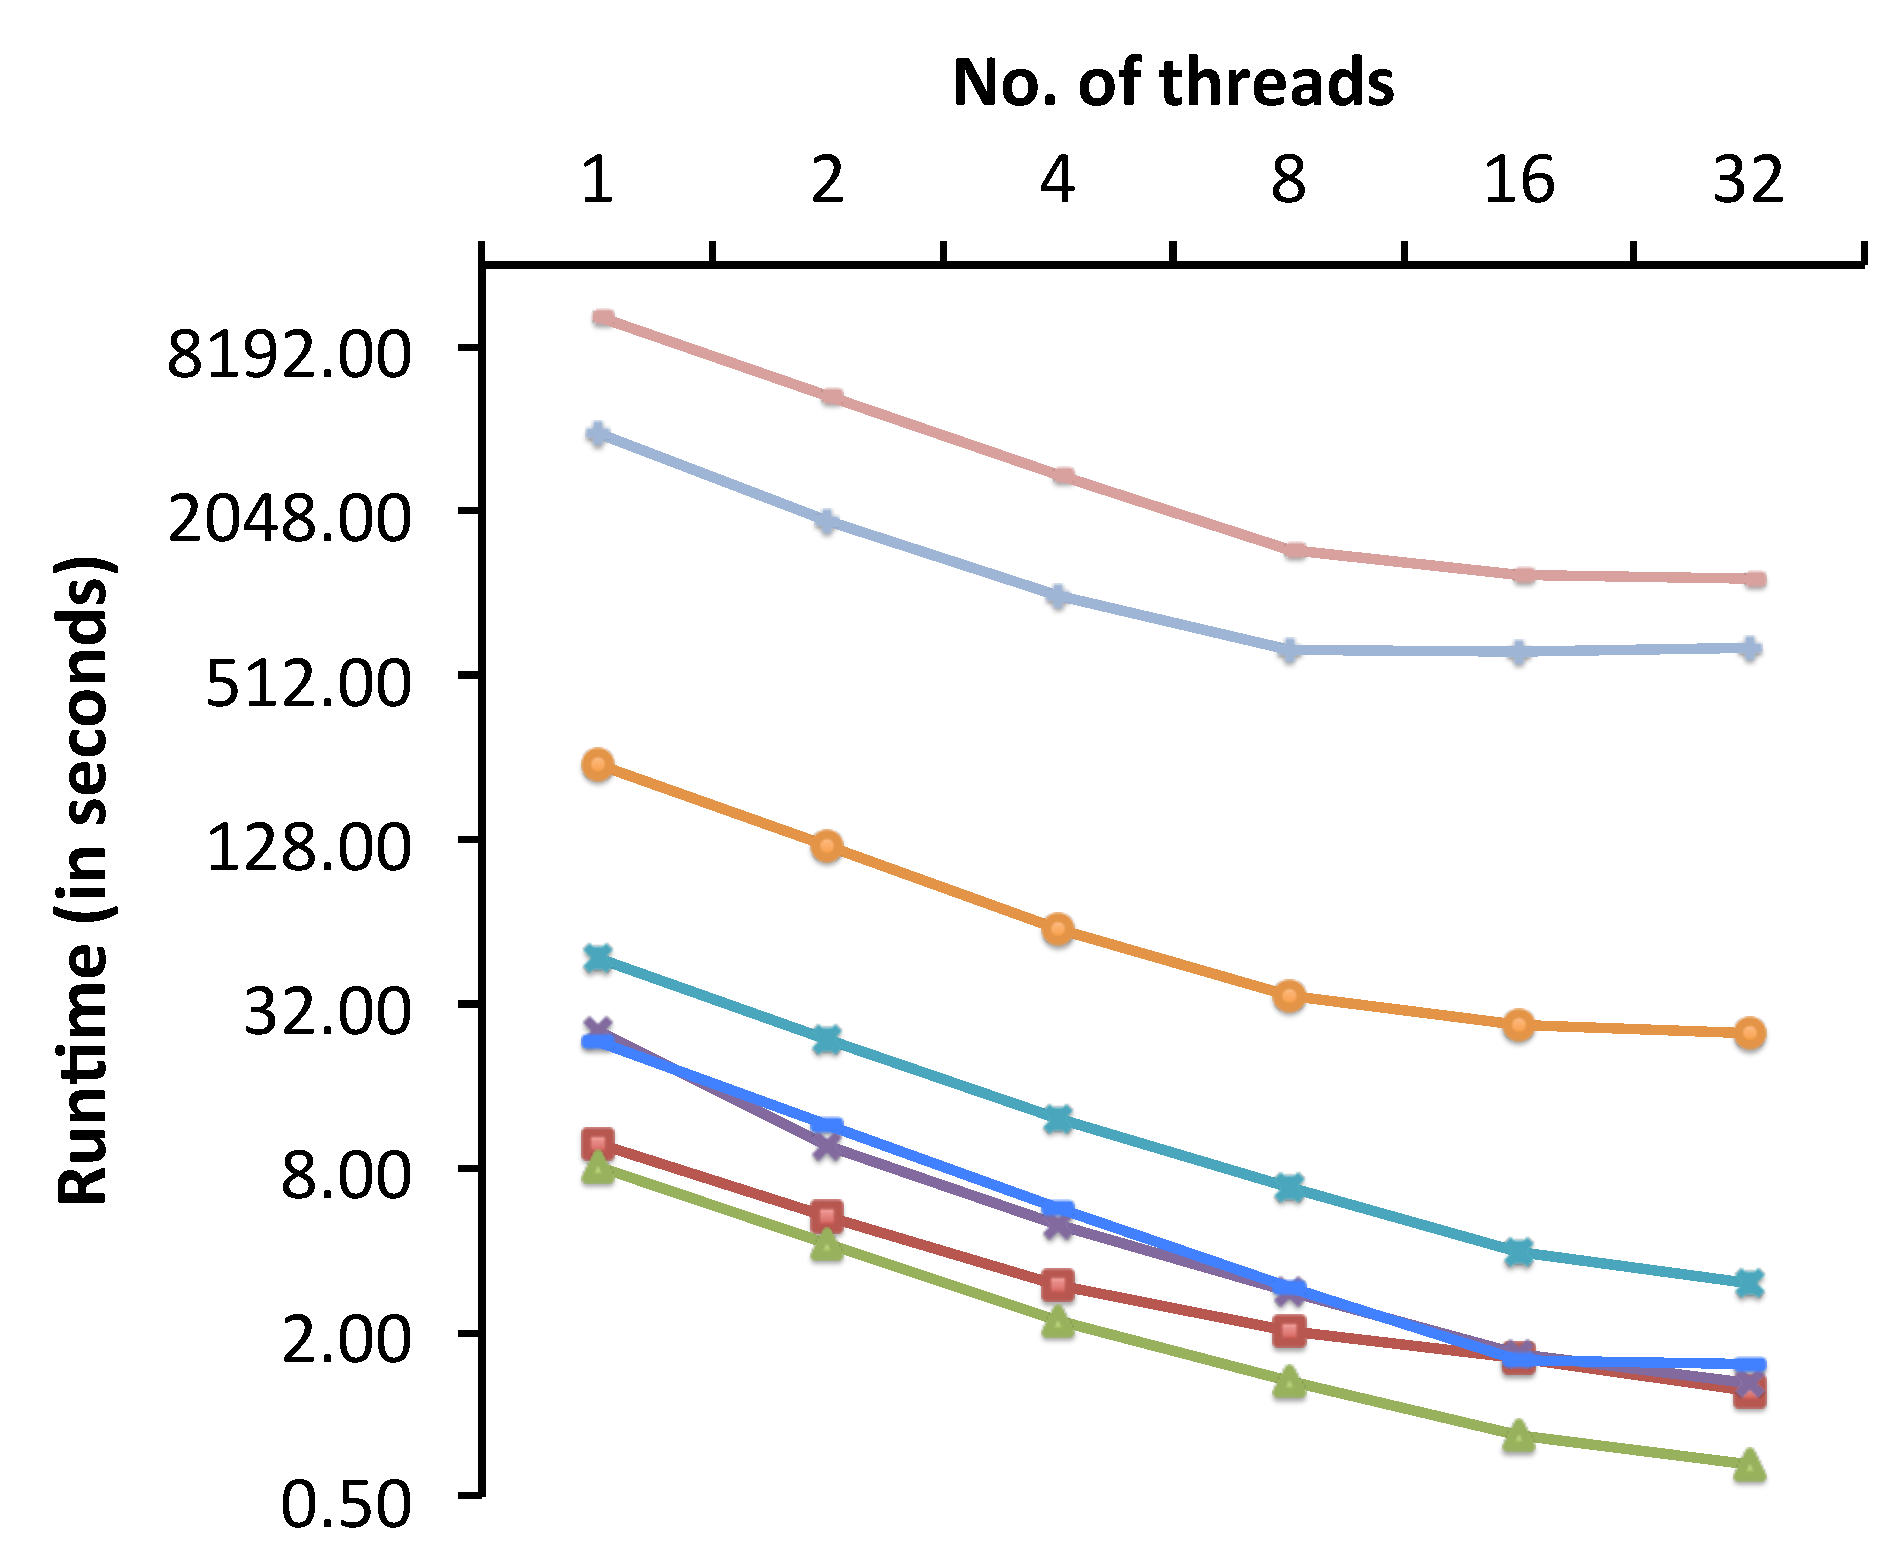
\includegraphics[width=\textwidth]{parallel_other_timing.pdf}
%                \caption{Timing results}
%                \label{fig:timing_realworld}
%        \end{subfigure}%
%        ~ %add desired spacing between images, e. g. ~, \quad, \qquad etc.
%          %(or a blank line to force the subfigure onto a new line)
%        \begin{subfigure}[b]{0.5\textwidth}
%                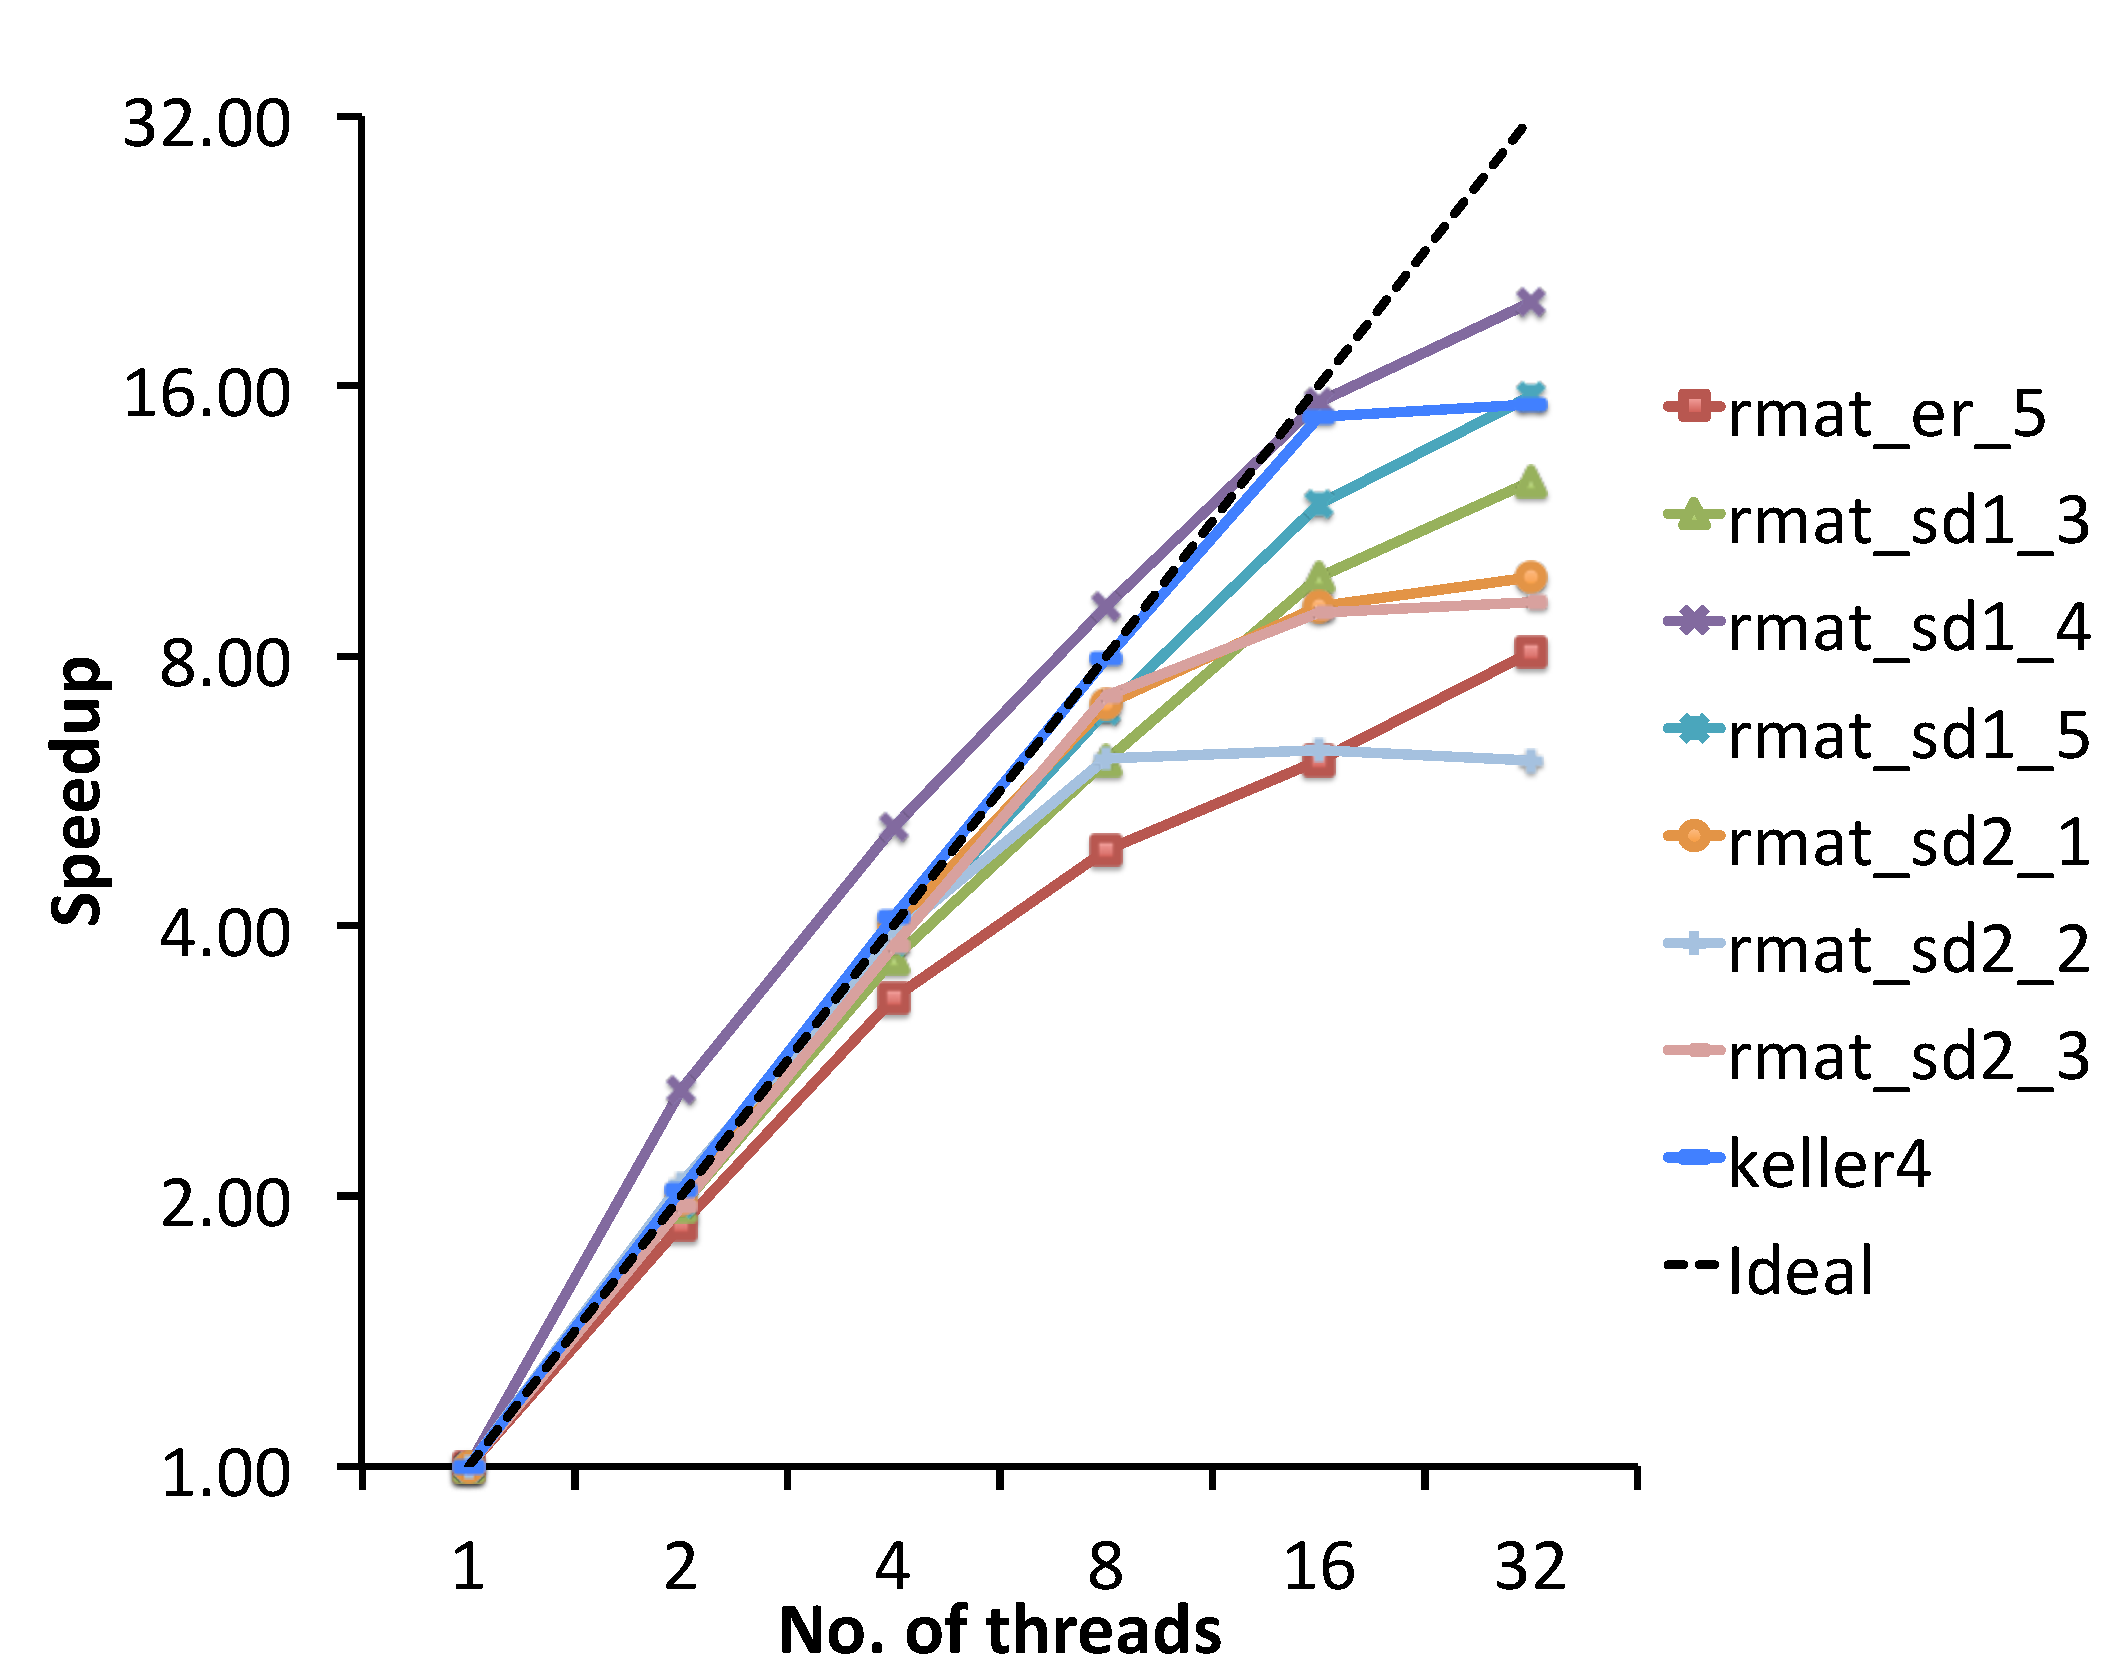
\includegraphics[width=\textwidth]{parallel_other_speedup.pdf}
%                \caption{Speedup results}
%                \label{fig:speedup_realworld}
%        \end{subfigure}
%        \caption{Performance of shared-memory parallelization on real-world graphs}\label{fig:parallel_perf}
%\end{figure}
%





